\PassOptionsToPackage{unicode=true}{hyperref} % options for packages loaded elsewhere
\PassOptionsToPackage{hyphens}{url}
%
\documentclass[]{article}

\usepackage{multirow}
\usepackage{graphicx}
\usepackage[]{algorithm2e}
% \usepackage{multirow}
 
 \usepackage[round]{natbib}
\usepackage{lmodern}

\usepackage{amssymb,amsmath}
\usepackage{ifxetex,ifluatex}
%\usepackage{fixltx2e} % provides \textsubscript
\ifnum 0\ifxetex 1\fi\ifluatex 1\fi=0 % if pdftex
  \usepackage[T1]{fontenc}
  \usepackage[utf8]{inputenc}
  \usepackage{textcomp} % provides euro and other symbols
\else % if luatex or xelatex
  \usepackage{unicode-math}
  
  \usepackage{hyperref}
  \usepackage{cleveref}
  \defaultfontfeatures{Ligatures=TeX,Scale=MatchLowercase}
\fi
% use upquote if available, for straight quotes in verbatim environments
\IfFileExists{upquote.sty}{\usepackage{upquote}}{}
% use microtype if available
\IfFileExists{microtype.sty}{%
\usepackage[]{microtype}
\UseMicrotypeSet[protrusion]{basicmath} % disable protrusion for tt fonts
}{}
\IfFileExists{parskip.sty}{%
\usepackage{parskip}
}{% else
\setlength{\parindent}{0pt}
\setlength{\parskip}{6pt plus 2pt minus 1pt}
}
\usepackage{hyperref}
\hypersetup{
            pdfborder={0 0 0},
            breaklinks=true}
\urlstyle{same}  % don't use monospace font for urls
\setlength{\emergencystretch}{3em}  % prevent overfull lines
\providecommand{\tightlist}{%
  \setlength{\itemsep}{0pt}\setlength{\parskip}{0pt}}
\setcounter{secnumdepth}{0}
% Redefines (sub)paragraphs to behave more like sections
\ifx\paragraph\undefined\else
\let\oldparagraph\paragraph
\renewcommand{\paragraph}[1]{\oldparagraph{#1}\mbox{}}
\fi
\ifx\subparagraph\undefined\else
\let\oldsubparagraph\subparagraph
\renewcommand{\subparagraph}[1]{\oldsubparagraph{#1}\mbox{}}
\fi
\usepackage{cleveref}
% set default figure placement to htbp
 
\def\fps@figure{htbp}
\makeatother


\author{Meng Lu }
%date{Feb 2021}
\title{An agent-based model for human activity simulation and the assessment of personal exposure to ambient air pollution}
\begin{document}
\maketitle
\begin{abstract}
 
 Long-term exposure assessment to spatiotemporally highly variable air pollutants requires accounting for human space-time activity behaviours. Current advancement in activity-based exposure assessment are either buffer-based, which is achieved through different level of spatial aggregation, or are agent-based, such as those integrating with transportation models. which are commonly parameterised using activity diaries. The advantage of using an agent-based approach in flexibly representing space-time activities is obvious. However, for the current agent-based models, there is a trade-off between the simulation accuracy and the ability of the model to scale to long-term, large population simulation, and separating between different population groups based on their socio-economical profiles. This trade-off is what the proposed agent-based model attempt to bridge. We develop an agent-based model specific for air pollution exposure assessment and explicitly account for uncertainty from activities through representing different activities and possible locations as random variables, which enable repeated random sampling. As the model does not rely on detailed GPS tracks or mobile diary surveys but any statistical mobility data, the model is applicable to different scales, as well as for large sub-population groups and long-term exposure assessment. The model consists of three independent modules: an activity simulation model, an air pollution prediction module, and an exposure calculation module that aggregates air pollution over the simulated space-time path based on the simulated activity schedules and the local environment of the locations. We demonstrate our model with the Dutch national mobile microcensus and high-resolution annually-average hourly NO$_2$ predicted from national ground stations. 

% in future, choose ABM dependsing on spatiotemporal variability of AP
% large-scale ABM with density functions. 
\end{abstract}

 
\section{Introduction}

%Chronic exposure to NO$_2$ poses a threat to public health, evidence has shown the negative effects of the NO$_2$ exposure to the cardiovascular and respiratory systems \citep{luo2016acute}. Despite public health concerns urging the attenuation of the negative effect of NO$_2$, the exact relationship between NO$_2$ exposure and our health remains unsolved. 
Highly traffic-related air pollutants such as NO$_2$ show considerable spatiotemporal variations at street levels. However, to understand the long-term or chronic health effects of NO$_2$ over a relatively large population (e.g. population of a city), most of epidemiological studies took a "static approach", which approximate the exposure as temporally averaged ambient pollutant concentrations at a person’s front-door home location. The same applies to risk assessment, the quantification of global, national, and local burden of diseases \citep{achakulwisut2019global}. It has been shown in many studies that for a spatiotemporally highly variable air pollutant, personal exposures assessed neglecting space-time activities, i.e. using concentration values at the front-door addresses, can differ considerably from personal exposures assessed accounting for human space-time activities \citep{duan1997combination,lu2019activity,park2017individual,molter2012performance,zenk2011activity}. \citep{yoo2015geospatial,yoo2021impact} took a step further to understand the joint effects of spatiotemporal mapping and space-time activities on exposure assessment, using respectively simulated and measured activity data. 

As measured activity data is hardly both over a long-term (e.g. a year or more) and a large population (e.g. millions). Activity simulation (commonly known as the "modelling approach") is needed. In transportation studies, progress has been made in the development of models for simulating transportation patterns, for example, the ALBATROSS \citep{ALBATROSS} is a transportation oriented system that simulates activities for the entire population based on activity diary data and dynamic constrains on scheduling decisions. Another relatively well-known activity simulation model is MATSim\citep{w2016multi}, which focuses on large-scale, one-day individual activity simulation based on a activity schedule scoring algorithm and detailed road networks. These activity models contribute to the understanding of human activity patterns \citep{miller2003prototype}. Many of these models are open-source \citep{w2016multi} and highly customisable, which allows scenario studies. The activity models consider a comprehensive set of space-time activity characters such as different travel means, work, education, and leisure activities, traffics \citep{w2016multi}. They are commonly parameterised by diary surveys consisting of locations visited and origin-destination schedules and estimate a continuous-time mobility track for each individual basing on general rules of human mobility patterns and space-time accessibility \citep{nguyen2011steps,gonzalez2008understanding,yang2010using,yu2006spatio,alessandretti2017multi,miller1991modelling}. Each route simulated can be contingent on, for instance, distance, safety, city infrastructure, and land use \citep{law2014measuring}. For example, \cite{shekarrizfard2017regional} assigned the predictions of a travel demand model to a road network to predict a person's hourly trajectories. For each person, the model selects a path from all possible paths by comparing the assigned travel time and the survey travel time. 


Integrating activity simulation models with predicted air pollution appear to be a solution to account for human space-time activities in exposure assessment. This has been reflected in several exposure studies \citep{shekarrizfard2017regional,deffner2016personal,gulliver2005time,dons2011impact}. A pioneered work is \cite{beckx2009dynamic}, who proposed to use the ALBATROSS to simulate hourly activities and then combine with an air dispersion model to assess exposure. However, none of these studies address long-term, uncertainty-quantified exposure assessment and for sub-populations. Specifically, \textit{long-term simulation} means the model is capable of quantifying exposure variations over longer times. \textit{Uncertainty} needs to be quantified for each simulated activity, including time schedules, travel modes, and possible destination locations. Separating \textit{sub population} groups allows more accurate simulation of their activities, as people's activity patterns may be clustered by their socio-economical status such as education, age, and occupation status. In another mindset, the confounders in health impacts studies such as age, gender, and living habits relate to certain space-time behaviours, but we only want to remove the effects of these confounders in health studies but not in exposure assessment, and this requires exposure assessment of sub-populations.  
%, which lead to bias in exposure assessment and thus the health study.

These three current limitations call for activity simulation models that are explicitly designed designed for exposure assessment. The framework developed in \cite{lu2019activity} attempts to address the first and second limitations. However, it assumes no activity information is available and therefore does consider population subgroups in real-life cases. We greatly extend from \cite{lu2019activity} to a new model which derives distributions of activity variables, namely travel modes and maximum travel distances, from national micro-census data. The proposed model estimates or empirically specifies probability distributions for each activity based on mobility surveys using statistical modeling for different population groups, and sampling from the specified or estimated distributions repeatedly for uncertainty quantification and more accurate estimation of exposures through ensembling. These allow the model to simulate closer to real-life exposures and greatly reduces uncertainty. 
    

With this novel space-time activity model as the core component, we develop an activity-based air pollution exposure assessment model consists of additionally an exposure calculation module and a temporal air pollution mapping module. The exposure calculation module takes the output of the activity model, namely activity schedules and spatial locations of the activities (e.g. work locations, trip routes), and hourly air pollution maps to assess exposures from each home location (\cref{fig:expflow}).     

\begin{figure}
    \centering
    \includegraphics[width=\linewidth]{figure/exposureflow.png}
    \caption{The structure of our exposure assessment model. At the core is the agent-based human space-time activity model. ABM: agent-based modelling. }
    \label{fig:expflow}
\end{figure}



We follow the ODD (Overview, Design concepts, and Details) protocol \citep[][page 37,]{railsback2019agent} to describe our agent-based model. Then, we show how the agent-based model is uses in our exposure assessment model and give an introduction to the exposure assessment model. We demonstrate the modelling process for exposure assessment in a study case. The activity model is implemented with the Dutch national micro-census data and the exposure is assessed in the Dutch city of Utrecht, for the population group university student.  %\Cref{sec:result} shows the results in our study case. \Cref{sec:dis} discuss our models and the results. \Cref{sec:con} closes with a conclusion.


\section{Model overview and design concepts }
\label{sec:model}

\subsection{Overview} 

\textbf{Purpose}:
The model is developed for large population-scale (e.g. The entire population of the Netherlands), long-term, personal air quality exposure assessment accounting for human space-time activities. For this purpose, the model is developed with three key features: 1) it can simulating long-term behaviours with abnormal events (e.g. holidays), 2) the uncertainty of human space-time activity is explicitly quantified, and 3) the activity simulation differs between population subgroups (e.g. with their age, sex, occupation status), which are separated in a way that between the groups the activity patterns are most distinct. %As the model is for large scale, we focus on deriving information from activity micro-survey data, in contrast to activity diaries and GPS tracks.% which may be employed for validation purposes. At a later stage, these data will be involved to dynamically improve the model.   

\textbf{Entities, state variables, and scales}:
The entities are each residence. The state variables include age, gender, education, occupation, income, working status (e.g. full-time worker or not), having children or not, and having a car or not.  The model is designed for long-term (one year or longer) exposure assessment over a population, focusing on a scale where land transportation (e.g. cars, bikes, on food) are the major commuting means. 

\textbf{Process overview}:

The most important task of the activity model is to generate activity schedules together with the spatial locations (\cref{fig:detail}) for each home locations.  In each interaction, the model sequentially sample or calculate the travel distances, the destination location, the travel mode, the  travel duration, the chosen of a free-time activity, and the start and end time of each activity. More specifically, the major steps are described as follows:   

\begin{enumerate}
    \item Specify the probability distribution of travel distances based on the mobility survey data if the distribution is not pre-defined. 
    \item Sample from the distribution of the travel distances to randomly sample a destination location from all possible destination locations.
    \item if within the sampled travel distance, there is no destination locations, the nearest destination location (based on the Euclidean distance) is chosen.  
    \item Based on the distance, the probability distribution of travel mode according to the relationships identified between travel mean and travel distances, for different population groups  (e.g. old people, students) and travel purposes (e.g. going to work), is used for sampling the travel model. 
    \item A route is queried from the road network for the sampled travel mode. For example, a walk path is queried if the travel mode is "on foot".  
    \item Based on the travel distances and the travel mode, the duration is deducted. 
    \item Based on the duration, the end time of a trip or the start time of the next trip is estimated. 
    \item If the previous trip is not on a road, the start time of the trip is generated with a distribution. For example, the default departure time to work in our model is sampled from a Gaussian distribution with mean 8 (i.e. 8 am) and standard deviation 0.2. 
    \item The free time activities are randomly sampled from a set of activities, for example, staying at home or take a walk. 
\end{enumerate}


 The process is repeated several times (each repetition is called an iteration) for uncertainty quantification and improving the prediction accuracy of the exposure assessment. 

\begin{figure}
    \centering
    \includegraphics[width=\linewidth]{figure/scheduleflow_noenrich.pdf}
  \caption{Procedure of generating activity schedules using the human space-time activity model}
    \label{fig:detail}
\end{figure}

\subsection{Design concepts}
The concept is to simulate personal space-time activities basing on probability sampling of agents' departure time, travel mode, maximum travel range, free-time activities, and possible destinations. The probability distributions (i.e. probability density function for continuous variables and probability mass function for discrete variables) can be empirically specified or derived mobility surveys with different socio-economical variables or other activity-related attributes (e.g. age) as covariates. The duration of working time is specified for different population groups (e.g. 8 hours for full-time workers). As the simulation results becomes closer to reality with more accurate probability distributions of the stochastic components, the population groups should be defined in a way that between them the activity patterns are most distinctive. The model can potentially be improved with high quality mobility survey and the integration of other mobility data.   This gives the model full flexibility of modelling and also for modelling at different spatial scales.     %This allows uncertainty quantification as well as a more accurate estimation of long-term behaviour through averaging. 


\subsection{Model Details}
\subsubsection{Input and output of the model}

The input of the activity model consists of 1) home locations to estimate, 2) all the possible destination locations for each destination type (e.g. all the work locations, all the school locations), and 3) the mobility survey. Alternatively, the mobility survey can be replaced by predefined probability distribution or probability distribution tables derived from the mobility survey for different population groups. In our demonstration example, we use a table for the probability each travel mode is taken for different distances and for different population groups and travel purposes, and a table for the distributions of the travel distances for each population groups.
 

The output of the activity model consists of activity schedules and corresponding spatial locations (including geospatial tracks) for each iteration and each individual. The activity schedule consists of, for each trip, a start time, an end time, the travel mode, the duration, as well as the activity name and a corresponding code (activity\_code in \cref{tab:sche}), which separates different free-time activities and links the schedule to the exposure assessment. \Cref{tab:sche} shows an example. Along with the spatial locations, the output also stores other properties of trips, including the speed, travel models, duration of a trip, the total number of locations a destination is drawing from.

\begin{table}[]
\resizebox{\textwidth}{!}{%
\begin{tabular}{cccccc}
\\[-1.8ex]\hline 
\hline \\[-1.8ex] 
start\_time & end\_time & activity   & activity\_code & travel\_mean          & duration                   \\ \hline
0.0         & 7.06      & home       & 1              & \multirow{7}{*}{foot} & \multirow{7}{*}{335.55672} \\
7.07        & 7.17      & h2w        & 2              &                       &                            \\
7.18        & 16.14     & work       & 3              &                       &                            \\
16.15       & 16.23     & w2h        & 2              &                       &                            \\
16.24       & 17.73     & home       & 1              &                       &                            \\
17.74       & 19.73     & free\_time & 1              &                       &                            \\
19.74       & 23.9      & home       & 1              &                       &     \\ \hline                      
\end{tabular}%
}
\caption{An example of simulated activity schedules. "h2w" means "home to work", and "w2h" means "work to home". The "duration" indicates the time that is used for for the activity in seconds. The integer part of the start and end times indicates hours, and the digits indicate minutes in percentage, e.g., 9.89 is at around 9:54 am (54 = 89*0.6). }
\label{tab:sche}
\end{table}

 %The model includes a built-in dataset of the Dutch national microcensus data called OViN. A description of the dataset is seen in \cref{sec:case}.


%The implementated population groups are: school student (U17) , University student (students older than 18 years old, Uni), part-time worker (PW), full-time worker (FW).


\subsubsection{Routing} 
Based on the transportation mode, the travel routes are queried from road networks constructed using the Python package OSMnx \citep{boeing2017osmnx}. The road network processes routes from OpenStreetMaps \citep{osmdata} into a network and removes the redundant nodes \citep{boeing2017osmnx}. This reduces the dataset size and accelerate route querying. There are three road types: "auto-vehicle", "bike", and "walk". The road network consists of an attribute travel time. For the travel model "auto-vehicle", the travel time is calculated in OSMnx, for the travel model "bicycle" and "on foot", the speed is assumed to be constant and can be specified by user, by default the speeds are set to 14 km/hr and 5 km/hr for bicycling and walking respectively. This allows selecting routes either based on the shortest distance or the shortest travel time. By default, we select a route based on the shortest travel time.  

\section{Exposure assessment model}
\label{sec:exp}
 
 Based the activity model and the temporal air pollution maps, the exposure calculation component aggregates over air pollution concentration over the spatial locations of the person. If the activity model is run $N$ time to simulate different schedules and spatial locations for each person, the  exposure is calculated $N$ times for the exposure of each iteration. By default, we use the mean of exposure calculated in the $N$ iterations as the final exposure assessed. The air pollution prediction model applies lightGBM (light gradient boosting machine) \citep{ke2017lightgbm} to each annually aggregated hourly air pollution measurements to predict air pollution. If temporal air quality maps are available, this module can be skipped. 
     
An activity-oriented view of the exposure calculated in a single iteration for two individuals is shown in \cref{exp_act}, which shows the activities, starting time, and the average exposure during the time-span of a certain activity.

\begin{figure}[!h]
    \centering
    \includegraphics[width=12cm]{figure/exposure_act1.png}
    \caption{Example of assessed average exposure during each activity, in a single simulation instance. The sub-plots show the average exposure calculated for each activity, and simply connect the two activities with a line, in contrast to plot the exposures continuously over time. The NO$_2$ exposure is in $\mu g/m^3$.}
    \label{exp_act}
\end{figure}


\subsubsection{Exposure calculation module}
\label{exposureassess}

The exposure assessment module queries and aggregates air pollution concentrations for each individual and over each activity in the activity schedule. We describe the process in pseudo-code \cref{pc_e} below: 
 
\begin{algorithm}[H]
 \KwData{temporal NO$_2$ maps, for each agent activity schedules and spatial locations associated with each activity in the schedule.}
 \KwResult{exposure assessed for each activity and for each person.}
 
 \For{each agent}{
 initialization\;
 exposure\_activity = 0 
 
 \For{each activity}{ 
    exposure\_activity $+=$ NO$_2$\_of\_corresponding\_time\_over spatial\_locations\_of\_the\_agent $\times$ activity\_duration
 }
exposure\_agent = exposure\_activity /time\_of\_all\_activities   
 }
 \caption{Exposure calculation, exposure\_agent indicates exposure calculated for each agent, exposure\_activity indicates exposure calculated for each activity in the schedule for each agent.}
 \label{pc_e}
\end{algorithm}


The exposure at home and at work are calculated as the air pollution concentration at the front door home and work locations multiplied to an indoor infiltration ratio, by default, this ratio is set to 0.7. Current implemented free-time activities include a) staying at home, b) in the garden or at terrace,  and c) taking a walk. The free-time activity b) is implemented as walking randomly within a distance (default 200m) close to the home location. The free-time activity c) is implemented as using a Gaussian kernel of distances away from home to the probability of being presence at the location (default, mean = 2000 m and standard deviation = 1 m).   

\section{Study case: activity modeling using the Dutch national microcensus data}

We demonstrate our model by simulating the exposure for the population group "university students" in Utrecht. The probability of travel mode and maximum travel range are derived from the Dutch national travel survey, OViN (2010 - 2017, followed by OVG and MON)). OViN is collected by Statistics Netherlands (in Dutch: Centraal Bureau voor de Statistiek - CBS) for one-day trip-based diary. It consists of 0.3\% of the Dutch population. We parse the text in the original dataset to extract the range of the data and calculate a mean of the data range. 

We simulate for the 49 university students who participated in the OViN survey and live in Utrecht at the time. The students are assumed to go to a university or college in the city during day-time and do some free-time activities (including staying at home) in the evening, a while after returning home. The departure time of going to the university of college is sampled from a Gaussian distribution with mean 9 (for 9 am) and standard deviation 1 (for 1 hour). The Departure time of leaving the university or college is sampled from a Gaussian distribution with mean 17 (for 5 pm) and standard deviation 1. All the university and college locations queried from OpenStreetMaps are used for all the destination locations. 
 
 
%The variables, their original text, and generated variables are listed in \cref{preprocess}.
% Please add the following required packages to your document preamble:
 
 
%   In our case-study (Utrecht) implementation, they are characterised from Dutch national activity surveys (OVin). The process is: 1) we select a profile (e.g. Univeristy student) and a purpose (e.g. go to work), 2) we fit the distribution of the selected data. 3) At each simulation, we sample one value from the distribution. Specifications are described below:


%Firstly, we characterise the distribution of the distances between home location and a work location. 
The destination location is determined in the following steps:     
\begin{itemize}
    \item Step 1: Distribution of travel distance. \\ From the histogram of the travel distances between the home location and school location (i.e. the Utrecht university or colleges) location \cref{stu_work_hist}, we can observe that the original distribution is log-normal or power law. The log transformed distribution becomes closer to a normal distribution. We therefore fit both models and at last decided on a log-normal. The Shapiro test indicates the log-transformed normal distribution is normal. 
    
    \item Step 2: Distance sampling. \\ In each simulation step, we sample a distance from the fitted log-normal distribution and this distance is considered as the maximum travel range.
    
    \item Step 3: Select candidate/potential destinations. \\ Destination locations within the Euclidean distance of the maximum travel range are considered as the "candidate destinations". As the actual routes have a longer distance, this can be seen as an a bit conservative way of selecting potential destinations. 
    
    \item Step 4: Randomly sample one location from all the potential destinations (\cref{buffer}).
    
\end{itemize}
\begin{figure}[!h]
    \centering
    \includegraphics[width=8cm]{figure/ditance_to_school.png}
    \caption{Histograms and density plots of the distances between students' home location to work locations. }
    \label{stu_work_hist}
\end{figure}

\begin{figure}[!h]
    \centering
    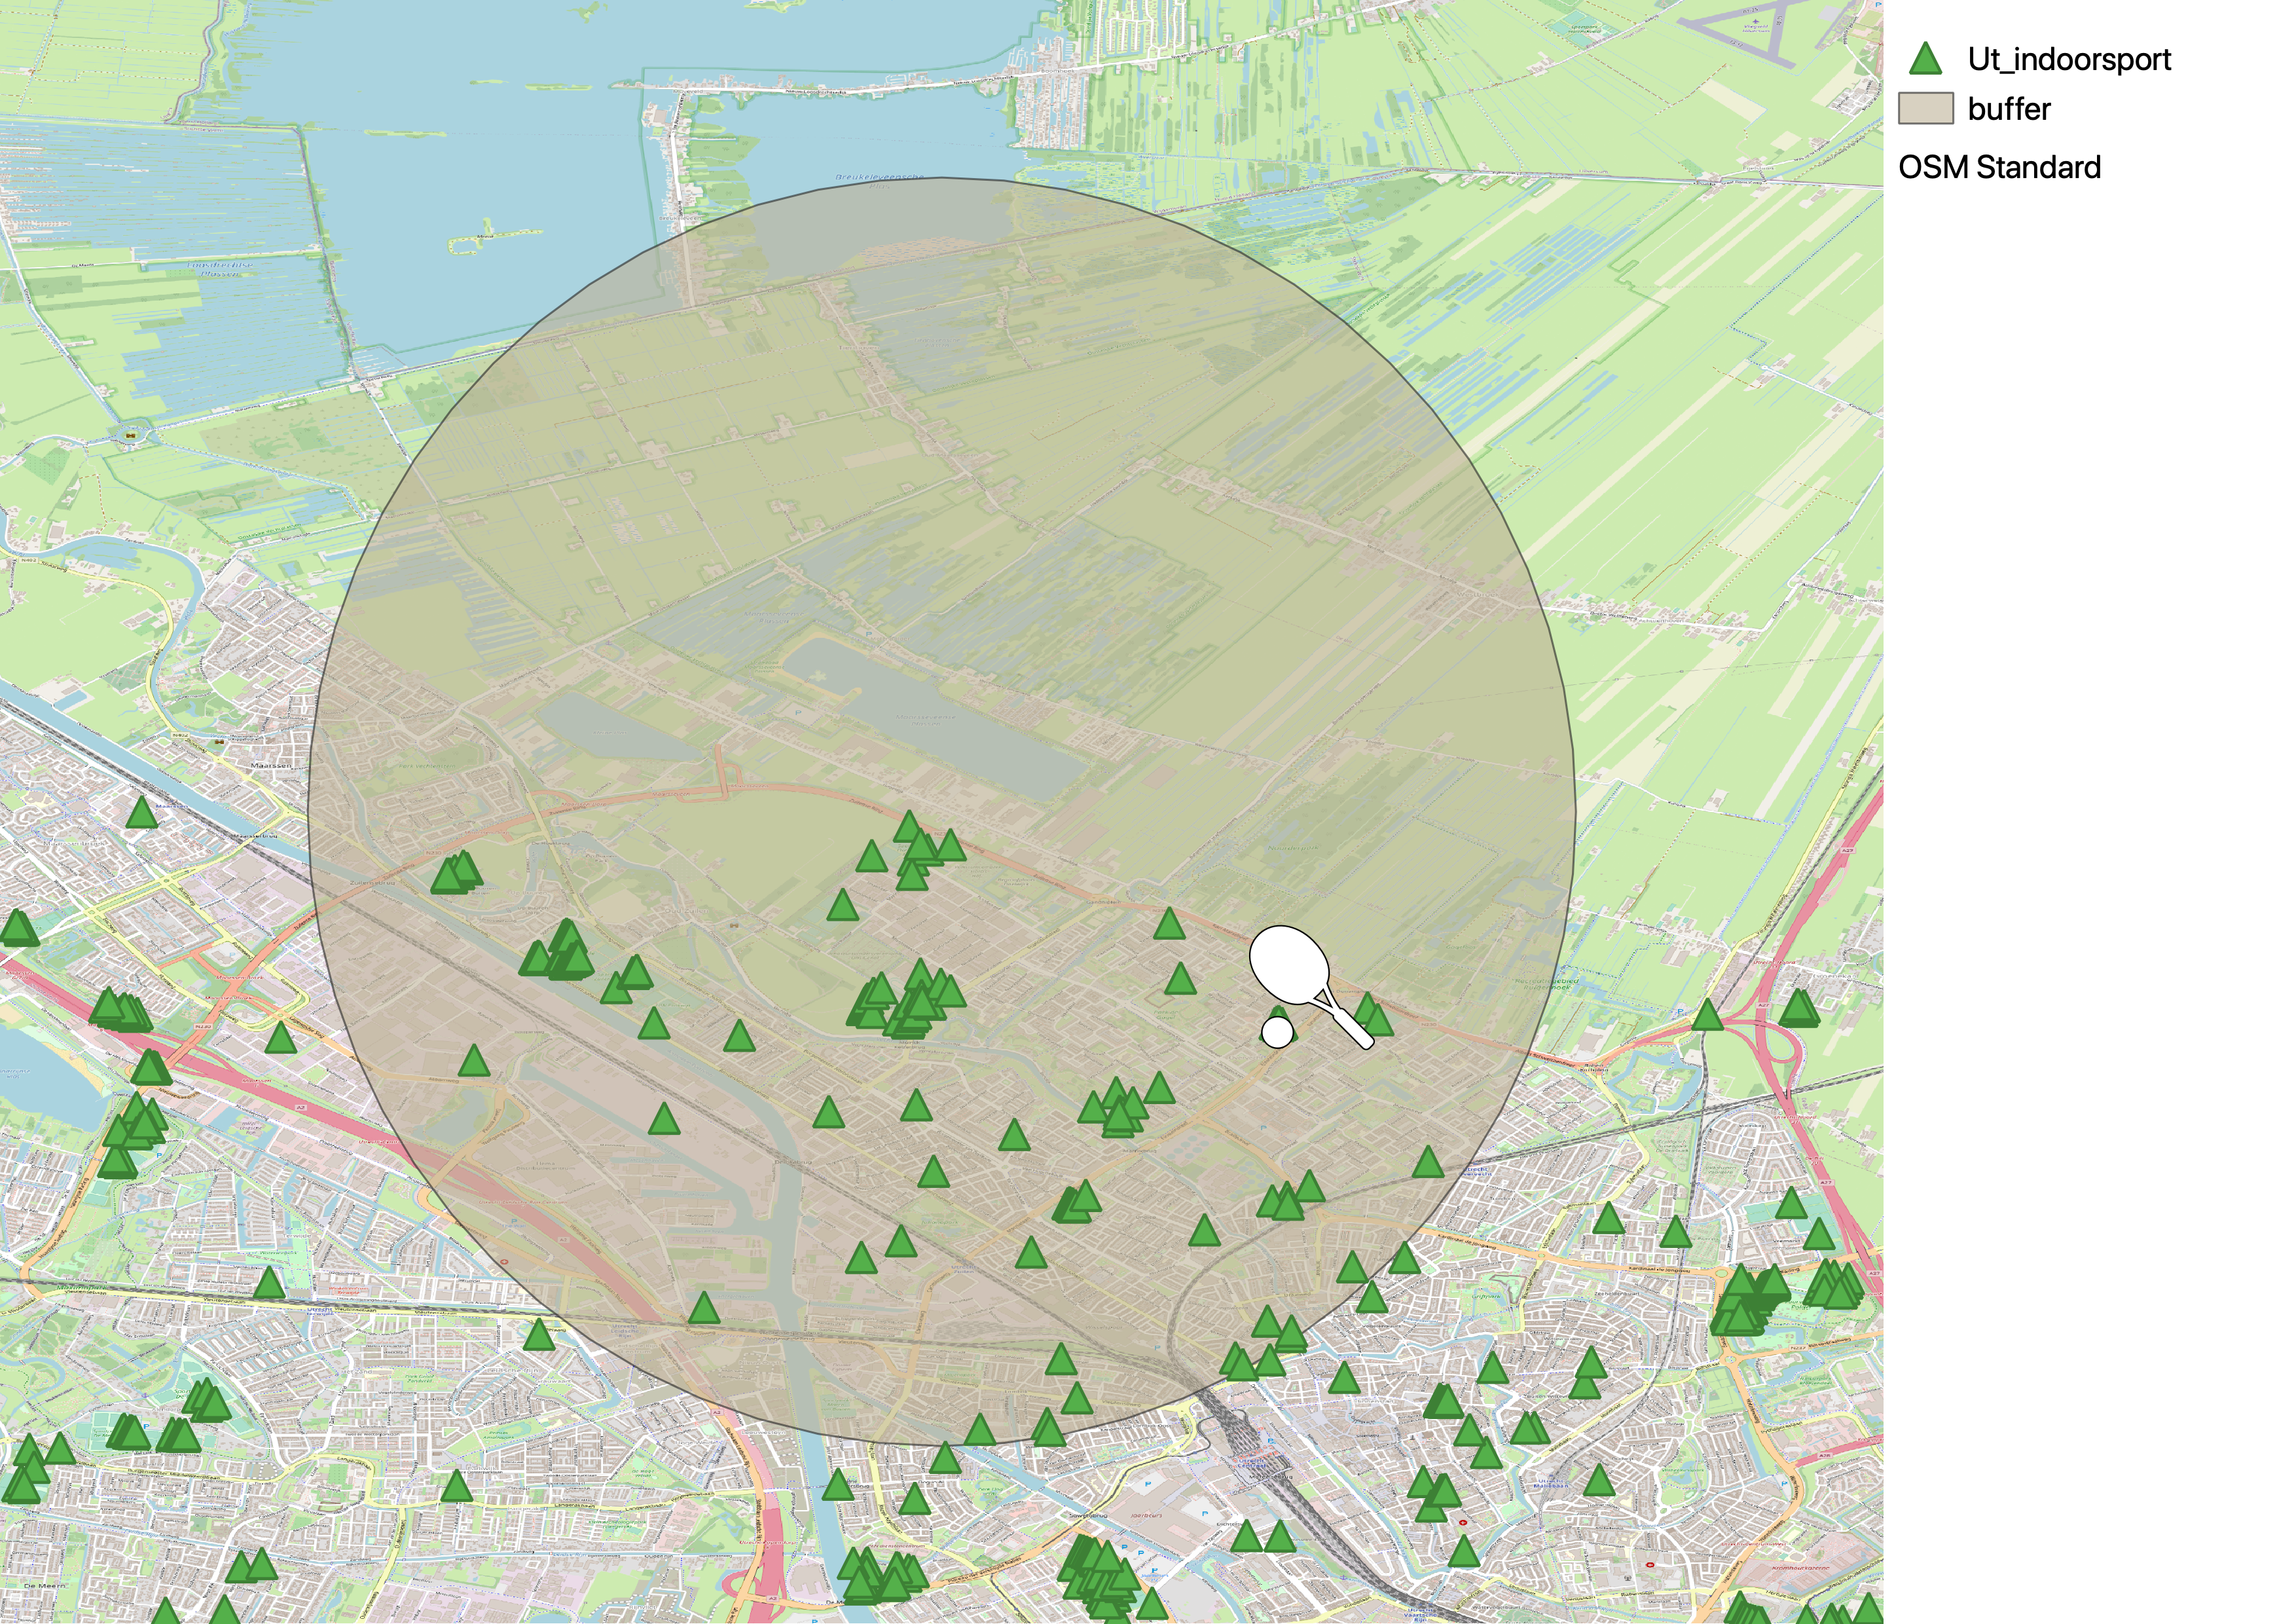
\includegraphics[width=8cm]{figure/buffer.png}
    \caption{Example of selecting a destination location. The triangles indicates all the possible destination locations (here: sports facilities). Only the locations within the maximum travel distances are considered, i.e. the green triangles within the buffer. And from them, one of the location is randomly sampled, marked as the \textit{Ping-pong racket and ball}. }
    \label{buffer}
\end{figure} 



\textbf{Choosing the transportation mode}

Now we have the home location and the destination (i.e. sport centre, school) locations, the second step is to choose the transportation mode based on the trip distance. 

\begin{itemize}
    \item Step 1: regroup transportation means and the travel distance range. \\ We regrouped the transportation means to walk, bicycle and auto-vehicle, which include all the other transportation vehicles (bus, tram, car,...). We regrouped the travel distance range as shown in \cref{stu_work_hist}. 
    
    \item Step 2: calculate the probabilities of the transportation means within each travel distance range. \\ we count for each travel distance range the incidence of each transportation mean, and divided by the total incidence of each travel distance range to obtain the probability (of the transportation mean in each travel distance range). The travel distance ranges are empirically defined in this study case and can be altered by users. 
    
    \item Step 3: sample the transportation mean. \\ 
    Based on the %walk distance (using the walking route queried using the OSMnx) 
    Euclidean distance between the origin and destination, we sample a transportation mean given the probabilities of taking a certain transportation method within the distance range.   
    
\end{itemize}



\begin{figure}[!h]
    \centering
    \includegraphics[width=8cm]{figure/ditance_vs_transmean_Uni.png}
    \caption{Probability of the transportation mean with regard to trip distance ranges for University students. The trip distance ranges are re-scaled from the original travel distance. The transportation means are re-grouped from the transportation means in the Ovin survey.}
    \label{Uni_mode_dist}
\end{figure}

\textbf{Generating the activity schedule and geospatial information (e.g. routes)}

 With the travel time to each destination, we can complete our schedule with the starting time and the ending time of each activity. There are two ways of generating the time of going to school, as described in the section \textit{Time Schedule} above. An example simulated schedules look like \cref{schedule}. An additional "Geometry" will be added to link the activity with the geographical points (e.g. front door location), lines (e.g. routes), or polygons (e.g. buffers). An example is shown in \cref{exampleroute}.
 
 
\begin{table}[!htbp] \centering 
  \caption{Example activity schedule 1, h2w means "home to work", and w2h means "work to home". The "bicycle" indicates the transportation mean, which is generated from the activity model. The integer part indicates hours, and the digits indicate minutes in percentage, e.g., 9.89 is at around 9:54 am. (54 = 89*0.6). } 
  \label{schedule} 
\begin{tabular}{@{\extracolsep{5pt}} cccc} 
\\[-1.8ex]\hline 
\hline \\[-1.8ex] 
 & start\_time & end\_time & activity \\ 
\hline \\[-1.8ex] 
1 & $0$ & $9.89$ & home \\ 
2 & $9.90$ & $10.19$ & h2w\_bicycle \\ 
3 & $10.20$ & $17.10$ & work \\ 
4 & $17.11$ & $17.39$ & w2h\_bicycle \\ 
5 & $17.40$ & $18.89$ & home \\ 
6 & $18.90$ & $19.89$ & sports \\ 
7 & $19.90$ & $23.90$ & home \\ 
\hline \\[-1.8ex] 
\end{tabular} 
\end{table}


\begin{figure}[!h]
    \centering
    \includegraphics[width=10cm]{figure/route.png}
    \caption{Example of routes queried from the OpenStreetMaps using the OSMnx, in the city of Utrecht. A route with the shortest travel time is selected. A: a bike route queried, B: a drive route, the background shows the network generated in OSMnx.}
    \label{exampleroute}
\end{figure}
%

We used the same official ground station measurements of Germany and Netherlands (all together 482 stations, with 66 stations in the Netherlands and 416 stations in Germany) to predict annual hourly NO$_2$ concentrations in Utrecht, for the year 2017. The geospatial predictors include road densities in different buffers (100, 300, 500, 1000, 3000, 5000 m) and of highways, primary roads, local roads from OpenStreetMaps, monthly wind speed and temperature of 2017 from ERA5-Land re-analysis, elevation of 90 m resolution, population from world pop, earth nightlight, radiation, and Sentinel 5p L3 product column density of 2018 (10 km resolution). 

The ensemble tree algorithm LightGBM \citep{ke2017lightgbm} is used for prediction. LightGBM is a tree-based gradient boosting framework, which uses histogram-based algorithms to bin the continuous values of each feature. The LightGBM obtained similar RMSE compared to XGBoost \citep{chen2015xgboost}, with optimised hyper-parameters. Different prediction patterns also affect the exposure assessment results \citep{yoo2021impact,yoo2015geospatial}, but is not the focus of this study. %We chose the algorithm based on our previous studies comparing the RMSE (Root Mean Squared Error) with the results of XGBoost \citep{chen2015xgboost}, with optimised hyper-parameters. We found the LightGBM obtained a slightly higher prediction accuracy (about 5\% lower in RMSE).
 
\subsubsection{Results}

\subsubsection{Annually aggregated hourly prediction of NO$_2$}

\Cref{con} shows hourly NO$_2$ predicted using Light GBM. The spatiotemporal dynamics of NO$_2$ could be clearly visible. These 24 maps are the input of the exposure calculation component. 

\begin{figure}[h]
    \centering
        \includegraphics[scale = 0.35]{figure/prediUt.png}
    \caption{Annually aggregated hourly NO$_2$ ($\mu g / m^3$) predicted for Utrecht.}
    \label{con}
\end{figure}


\Cref{sims} shows an example of exposure assessed in several iterations for a subset of university students in Utrecht (\cref{sims}) who participated in the OViN survey. The exposure assessed using true location is shown for comparison. It can be observed that the exposure calculated using the proposed model is close to the exposure calculated using the true location. The exposure assessed in multiple iterations provide us with an uncertainty measure. We only ran three iterations for the visualisation purposes, in reality, more iterations lead to a more accurate uncertainty estimation, as well as the exposure prediction (e.g. by taking the mean). 

\begin{figure}[h]
    \centering
    \includegraphics[width=8cm]{figure/sims.png}
    \caption{Exposure assessed for 30 university students. The exposure is calculated as aggregating the NO$_2$ concentration along the route over the corresponding time span. The red dots indicate exposure assessed using real location, and others 3 times of simulated university locations and travel means.}
    \label{sims}
\end{figure}


\Cref{expmap} shows the exposure assessed using the proposed simulation model for the 49 university students, with 11 iterations as recommended in \citep{lu2019activity}. It can be observed that high exposures do not necessarily occur for people with high concentrations at the front door home locations. Note that with university students, the uncertainty in choosing the destination location is relatively low compared to for example full-time workers, as the number of university or colleagues in a city is limited. 

\begin{figure}[h]
    \centering
    \includegraphics[width=8cm]{figure/utschoolmean2.pdf}
    \caption{Exposure assessed for the population group university students, using the mean of the 11 iterations.  Background: annual mean NO$_2$ prediction for 2017, calculated by taking the average of all the annual hourly NO$_2$ predictions.}
    \label{expmap}
\end{figure}

 

\section{Discussion}
\label{sec:dis}


%An alternative way to replace step 3 and 4 in destination location selection is to calculate the distances between the original location and all the destination locations, and directly sample a location. This method is computationally much more intensive. 



We have focused on describing and demonstrating of our space-time activity model, as well as how it is used together with the air prediction and the exposure calculation components for exposure assessment. The Dutch micro-census data is used to parameterise our model and a study case is shown for the assessment of NO$_2$ exposed by university students in Utrecht. The differences between using the front-door location concentrations and our simulation model, as well as using the real locations, are clearly visualised. 

A major improvement of our activity model compared to recent activity-based exposure assessment models \citep{lu2019activity} is that it proposes the location and schedule simulation algorithms being explicitly basing on the probability distributions of the variables (e.g. the travel mode and the maximum travel range) that determines the activity patterns of different population groups. Also, the departure times, free time activities, and the time for starting the free-time activities can all be sampled from a specific probability distribution. These greatly reduce the uncertainty in the activity simulation in general and for different population groups, which make it more suitable to be used in health studies and risk assessment. Compared to the proposed model, the framework of \citep{lu2019activity} consists of a complete random destination sampling procedure, a static activity schedule, and assumes one travel mode for all the simulation iterations. We believe the the proposed model does not sacrifice the generality with a much confined sampling space and more stochastic components. 


%The model simulation for routes and schedules is fast, the only costly function is the nearest point searching. %

Our model relies on the distribution of the variables of travel behaviours and is therefore flexible and scalable. It is flexible as it can potentially include any variables  influencing the travel behaviour. For example, the probability of selecting a travel mean could be estimated using the relationships with other variables such as a classification map indicating the rural, suburban, and urban land-use, the weather conditions, the emission regulations, or fuel price, additional to the characters of the individual as has been shown in our study case (based on e.g. age or if a person is a student or a worker). The model is scalable means the model can be applied to any areas as long as the mobility information (e.g. at the micro-census data level) is sufficient for the area. By design, the model focuses on land travel behaviour, i.e. we don't consider taking flight or long-distance ferries. The current model consider travel by train the same as travel by auto-vehicles (e.g. car, bus), in future we aim at a more sophisticated design for the train profile. 

 % Note: How is the train route calculated? If an agent (person) takes
  %a train, it is assumed he/she will firstly walk or cycle to the
  %nearest train station, and get off at the train station closest to the
  %destination location. (\emph{to be considered}). I intend to firstly
  %model within the Utrecht city, so all the destinations should be
  %constrained to a certain distance, therefore the mode: train has a
  %very small probability. This model may also be remove, then in
  %implementation i can simply replace train with autovehicles  .
  
  In choosing the travel mode, we used Euclidean distance between the departure and arrival locations, and therefore may be more likely to choose a lower-speed traffic mode (e.g. on foot than by bicycle). The reason for using Euclidean distance instead of the road distance is to avoid additional route querying, which takes longer computation time. Commonly, the Euclidean distance becomes closer to the road distance with increased travel distance. As the model is developed to simulate for a large population, multiple populations, and multiple iterations, the computational cost is a concern.
 
    
The exposure calculation model iterates over each person and then aggregate the air pollution concentrations over the route of each activity of the person (with the indoor-outdoor ratio accounted). It is highly parallelisable as the exposure calculation is independent for each individual. Note the individuals could still interact to each other and with the environment when simulating the route and the schedules. Another way of calculating the exposure is to iterate over each time step, i.e., for each time step, the exposure of the entire population is calculated. This way can be parallelised for each time step instead of each individual. For a population larger than the number of time steps, this way may provide an efficient alternative.  

The modelling concept can potentially be applied to other exposure assessment tasks, for example Ozone and Particulate Matters. The model is easy to use and be extended to enable different interactions and complex scenarios. As the probability distributions are mainly derived statistically, diverse data sources could be easily assimilated. Sophisticated statistical modelling can be used to predict the probability density or mass functions, with uncertainty quantified and integrated in the exposure assessment model. The interdisciplinary contributions are also facilitated as the statistical analysis could be independently carried out without the knowledge of the entire exposure assessment model. 

\section{Conclusion}
\label{sec:con}

We developed an activity-based personal exposure assessment model for long-term exposure assessment of different population groups. The core of it is an agent-based activity simulation model, the key concept of it is to repeatedly sample from a probability density function or a probability mass function of the variable (e.g. travel mode) that determines the activity patterns. The personal exposure is repeatedly assessed in multiple iterations to allow uncertainty quantification and improve the prediction. The probability density or mass functions can be derived from any mobility data, or a combination of them, with any predictive model, which make the model extensive and easily scalable spatially. We used the Dutch national micro-census survey to demonstrate our model and showed the exposure assessed using our model with simulated and known destination locations for the population group university (and colleague) students. The result shows the differences between modelling and not modelling space-time activities in exposure assessment, as well as how the uncertainty in exposure could be quantified with our model. 


\newpage
\bibliographystyle{plainnat}
\bibliography{ref}


\end{document}

\begin{table}[!htbp] \centering 
  \caption{Example activity schedule 2, for notations please refer to \cref{schedule}. "Auto" indicates all the other vehicles, of course, for U17, they are not driving themselves.} 
  \label{schedule2} 
\begin{tabular}{@{\extracolsep{5pt}} cccc} 
\\[-1.8ex]\hline 
\hline \\[-1.8ex] 
 & start\_time & end\_time & activity \\ 
\hline \\[-1.8ex] 
1 & $0$ & $9.33$ & home \\ 
2 & $9.34$ & $9.60$ & h2w\_auto \\ 
3 & $9.61$ & $16.43$ & work \\ 
4 & $16.44$ & $16.69$ & w2h\_auto \\ 
5 & $16.70$ & $18.19$ & home \\ 
6 & $18.20$ & $19.19$ & sports \\ 
7 & $19.20$ & $23.90$ & home \\ 
\hline \\[-1.8ex] 
\end{tabular} 
\end{table} 


\subsection{Implementation}
\begin{enumerate}
\def\labelenumi{\arabic{enumi}.}
\item
  Activities:
  \emph{Work-day activities:} 1) home, 2) home to work, 3) work, 4) work
  to home, 5) sports. The assumption for sports is that it occurs in the
  morning or evening, and it occurs either 1 hour before departure to
  work or 1 hour after come back home from work.

  \emph{Weekend activity}: 1) shopping, 2) random walk 
\item
  A \textbf{probailistic} model: the components below are probabilistic,
  and the densities can come for activity surveys or literature.

  1) \underline{Time schedule:} please see section 2 for the activities.
  The departure times to work and back from home are probabilisitic. By
  default, a gaussian distribution is used (e..g with mean 8 and
  standard deviation 0.5 for going to work). In our implementation, the
  distributions of departure times are fitted (characterised) from human
  activity surveys (please see section 4 below). The distributions are
  fitted for each population group.

  2) \underline{Unknown destination locations:} For large-population
  activity modeling, it is commonly the case that the specific
  destination location (e.g. work location, sport centres) are unknown
  for each individual. However, the information for the entire locations
  (e.g. sport centres, work buildings, universities, schools) are
  becoming more comprehensive. In many countries, this part of
  information can be acquired from OpenStreetMaps. In this study, we
  select potential locations by proabilisticly sampling the maximum trip
  distance and only randomly select locations within the Euclidean
  distance of the maximum trip distance. If there is no destination
  points within the sampled maximum trip distance, the nearest
  destination point is used. The number of total selected destination
  points serve as an uncertainty indicator in the situation of unknown
  destination locations, in each simulation run.

  3) \emph{\underline{Means of commuting}} (currently: (train),
  autovehicles (car, bus, tram), bike, on foot): are deteremined based
  on travel distance. Based on the population group (e.g. school
  student) and the travel purpose (to school), the probability that a
  certain travel mean is taken is calculated (e.g. 0.3 for on foot and
  0.6 for biking, 0.1 for taking a bus or car and 0 for others),
  according to which a travel mode is sampled in each simulation. The
  commuting routes are queried from OpenStreetMaps.

  Note: {[}How is the train route calculated? If an agent (person) takes
  a train, it is assumed he/she will firstly walk or cycle to the
  nearest train station, and get off at the train station closest to the
  destination location. (\emph{to be considered}). I intend to firstly
  model within the Utrecht city, so all the destinations should be
  constrained to a certain distance, therefore the mode: train has a
  very small probability. This model may also be remove, then in
  implementation i can simply replace train with autovehicles{]} .
\item
  Implementation:

  Population group implemented are: school student (U17) , University
  student (students older than 18 years old, Uni), part-time worker
  (PW), full-time worker (FW).

  There is a conceptural default implemented in our model which is
  described in table 1. In our case-study (Utrecht) implementation, they
  are characterised from Dutch national activity surveys (OVin). The
  process is: 1) we select a profile (e.g. Univeristy student) and a
  purpose (e.g. go to work), 2) we fit the distribution of the selected
  data. 3) At each simulation, we sample one value from the
  distribution. Specifications are described below:

  \textbf{Destination location selection:}
\end{enumerate}



  \textbf{Destination location selection:}
\begin{itemize}
\item
  Default: randomly pick a location.
\item
  OVin: probability counted from means of \emph{commuting vs. distance}.
  for each population group (but not specified with travel purpose).
\item
  Profile implemented: School students (U17), University students (Uni),
  PW, FW; for going to work (including all functional non-residential
  buildings, data same as the Utrecht paper), going to universities
  ((locations from OSM), going to schools (locations from OSM).

  \textbf{Means of commuting}:
\item
  Default: conceptural probabilistic model for going to work.
\item
  OVin: probability counted from means of \emph{commuting vs. distance}.
  for each population group (but not specified with travel purpose).
\item
  Profile implemented: School students (U17), University students (Uni),
  PW, FW.

  \textbf{Departure time to work:} 
\item
  Default: gaussian model with mean 8 and standard deviation (SD) 0.5.
\item
  OVin: Distribution characterised: departure time (KVtijd). 
\item
  Profile implemented \emph{(Todo)}: School students (U17), University
  students (Uni), PW, FW. 
\end{itemize}
\label{sec:case}
The example below shows how we model the profile group: school student (U17). The activities considered are 1) going to school, 2) staying at school, 3) going back home, 4) going to a sport center, 5) going back home.  


\begin{enumerate}
\def\labelenumi{\arabic{enumi}.}
%\item
%  Activities:  \emph{Work-day activities:} 1) home, 2) home to work, 3) work, 4) work
%  to home, 5) sports. The assumption for sports is that it occurs in the
%  morning or evening, and it occurs either 1 hour before departure to
%  work or 1 hour after come back home from work.

%  \emph{Weekend activity}: 1) shopping, 2) random walk 
\item
  A \textbf{probailistic} model: the components below are probabilistic,
  and the distributions can come for activity surveys or literature.

  1) \underline{Time schedule:} please see section 2 for the activities.
  The departure times to work and back from home are probabilisitic. By
  default, a gaussian distribution is used (e..g with mean 8 and
  standard deviation 0.5 for going to work). In our implementation, the
  distributions of departure times are fitted (characterised) from human
  activity surveys (please see section 4 below). The distributions are
  fitted for each population group.

  2) \underline{Unknown destination locations:} For large-population
  activity modeling, it is commonly the case that the specific
  destination location (e.g. work location, sport centres) are unknown
  for each individual. However, the information for the entire locations
  (e.g. sport centres, work buildings, universities, schools) are
  becoming more comprehensive. In many countries, this part of
  information can be acquired from OpenStreetMaps. In this study, we
  select potential locations by probabilisticly sampling the maximum trip
  distance and only randomly select locations within the Euclidean
  distance of the maximum trip distance. If there is no destination
  points within the sampled maximum trip distance, the nearest
  destination point is used. The number of total selected destination
  points serve as an uncertainty indicator in the situation of unknown
  destination locations, in each simulation run.

  3) \emph{\underline{Means of commuting}} (currently: (train),
  autovehicles (car, bus, tram), bike, on foot): are deteremined based
  on travel distance. Based on the population group (e.g. school
  student) and the travel purpose (to school), the probability that a
  certain travel mean is taken is calculated (e.g. 0.3 for on foot and
  0.6 for biking, 0.1 for taking a bus or car and 0 for others),
  according to which a travel mode is sampled in each simulation. The
  commuting routes are queried from OpenStreetMaps.
 

\end{enumerate}



\begin{table}[!h]
\resizebox{\textwidth}{!}{%
\begin{tabular}{l|l|l|l|l|l}
\hline
Variable       & original variable name & \begin{tabular}[c]{@{}l@{}}example of the \\ variable content\end{tabular}                           & new variables                                                                     & \begin{tabular}[c]{@{}l@{}}new \\ variable\\  value\end{tabular} & note                                                                                                                                                              \\ \hline
Trip distances & KAfstR                 & \begin{tabular}[c]{@{}l@{}}"5,0 tot 7,5 km"\\ "50 km of meer"\\ "Geen rit in Nederland"\end{tabular} & \begin{tabular}[c]{@{}l@{}}KAf\_low\\ KAf\_mean\\ KAf\_high\end{tabular} & \begin{tabular}[c]{@{}l@{}}5\\ 6.25\\ 7\end{tabular}             & \begin{tabular}[c]{@{}l@{}}"geen rit in\\  Nederland" \\ means the trip \\ is not in the \\ Netherlands \\ and is not \\ considered \\ in this study\end{tabular} \\ \hline
Income         &                        &                                                                                                      &                                                                                   &                                                                  &                                                                                                                                                                   \\ \hline
Age            &                        &                                                                                                      &                                                                                   &                                                                  &                                                                                                                                                                   \\ \hline
...            &                        &                                                                                                      &                                                                                   &                                                                  &                                                                                                                                                                   \\ \hline
\end{tabular}%
}
\label{preprocess}
\end{table}